\documentclass[11pt]{article}

    \usepackage[breakable]{tcolorbox}
    \usepackage{parskip} % Stop auto-indenting (to mimic markdown behaviour)
    

    % Basic figure setup, for now with no caption control since it's done
    % automatically by Pandoc (which extracts ![](path) syntax from Markdown).
    \usepackage{graphicx}
    % Keep aspect ratio if custom image width or height is specified
    \setkeys{Gin}{keepaspectratio}
    % Maintain compatibility with old templates. Remove in nbconvert 6.0
    \let\Oldincludegraphics\includegraphics
    % Ensure that by default, figures have no caption (until we provide a
    % proper Figure object with a Caption API and a way to capture that
    % in the conversion process - todo).
    \usepackage{caption}
    \DeclareCaptionFormat{nocaption}{}
    \captionsetup{format=nocaption,aboveskip=0pt,belowskip=0pt}

    \usepackage{float}
    \floatplacement{figure}{H} % forces figures to be placed at the correct location
    \usepackage{xcolor} % Allow colors to be defined
    \usepackage{enumerate} % Needed for markdown enumerations to work
    \usepackage{geometry} % Used to adjust the document margins
    \usepackage{amsmath} % Equations
    \usepackage{amssymb} % Equations
    \usepackage{textcomp} % defines textquotesingle
    % Hack from http://tex.stackexchange.com/a/47451/13684:
    \AtBeginDocument{%
        \def\PYZsq{\textquotesingle}% Upright quotes in Pygmentized code
    }
    \usepackage{upquote} % Upright quotes for verbatim code
    \usepackage{eurosym} % defines \euro

    \usepackage{iftex}
    \ifPDFTeX
        \usepackage[T1]{fontenc}
        \IfFileExists{alphabeta.sty}{
              \usepackage{alphabeta}
          }{
              \usepackage[mathletters]{ucs}
              \usepackage[utf8x]{inputenc}
          }
    \else
        \usepackage{fontspec}
        \usepackage{unicode-math}
    \fi

    \usepackage{fancyvrb} % verbatim replacement that allows latex
    \usepackage{grffile} % extends the file name processing of package graphics
                         % to support a larger range
    \makeatletter % fix for old versions of grffile with XeLaTeX
    \@ifpackagelater{grffile}{2019/11/01}
    {
      % Do nothing on new versions
    }
    {
      \def\Gread@@xetex#1{%
        \IfFileExists{"\Gin@base".bb}%
        {\Gread@eps{\Gin@base.bb}}%
        {\Gread@@xetex@aux#1}%
      }
    }
    \makeatother
    \usepackage[Export]{adjustbox} % Used to constrain images to a maximum size
    \adjustboxset{max size={0.9\linewidth}{0.9\paperheight}}

    % The hyperref package gives us a pdf with properly built
    % internal navigation ('pdf bookmarks' for the table of contents,
    % internal cross-reference links, web links for URLs, etc.)
    \usepackage{hyperref}
    % The default LaTeX title has an obnoxious amount of whitespace. By default,
    % titling removes some of it. It also provides customization options.
    \usepackage{titling}
    \usepackage{longtable} % longtable support required by pandoc >1.10
    \usepackage{booktabs}  % table support for pandoc > 1.12.2
    \usepackage{array}     % table support for pandoc >= 2.11.3
    \usepackage{calc}      % table minipage width calculation for pandoc >= 2.11.1
    \usepackage[inline]{enumitem} % IRkernel/repr support (it uses the enumerate* environment)
    \usepackage[normalem]{ulem} % ulem is needed to support strikethroughs (\sout)
                                % normalem makes italics be italics, not underlines
    \usepackage{soul}      % strikethrough (\st) support for pandoc >= 3.0.0
    \usepackage{mathrsfs}
    

    
    % Colors for the hyperref package
    \definecolor{urlcolor}{rgb}{0,.145,.698}
    \definecolor{linkcolor}{rgb}{.71,0.21,0.01}
    \definecolor{citecolor}{rgb}{.12,.54,.11}

    % ANSI colors
    \definecolor{ansi-black}{HTML}{3E424D}
    \definecolor{ansi-black-intense}{HTML}{282C36}
    \definecolor{ansi-red}{HTML}{E75C58}
    \definecolor{ansi-red-intense}{HTML}{B22B31}
    \definecolor{ansi-green}{HTML}{00A250}
    \definecolor{ansi-green-intense}{HTML}{007427}
    \definecolor{ansi-yellow}{HTML}{DDB62B}
    \definecolor{ansi-yellow-intense}{HTML}{B27D12}
    \definecolor{ansi-blue}{HTML}{208FFB}
    \definecolor{ansi-blue-intense}{HTML}{0065CA}
    \definecolor{ansi-magenta}{HTML}{D160C4}
    \definecolor{ansi-magenta-intense}{HTML}{A03196}
    \definecolor{ansi-cyan}{HTML}{60C6C8}
    \definecolor{ansi-cyan-intense}{HTML}{258F8F}
    \definecolor{ansi-white}{HTML}{C5C1B4}
    \definecolor{ansi-white-intense}{HTML}{A1A6B2}
    \definecolor{ansi-default-inverse-fg}{HTML}{FFFFFF}
    \definecolor{ansi-default-inverse-bg}{HTML}{000000}

    % common color for the border for error outputs.
    \definecolor{outerrorbackground}{HTML}{FFDFDF}

    % commands and environments needed by pandoc snippets
    % extracted from the output of `pandoc -s`
    \providecommand{\tightlist}{%
      \setlength{\itemsep}{0pt}\setlength{\parskip}{0pt}}
    \DefineVerbatimEnvironment{Highlighting}{Verbatim}{commandchars=\\\{\}}
    % Add ',fontsize=\small' for more characters per line
    \newenvironment{Shaded}{}{}
    \newcommand{\KeywordTok}[1]{\textcolor[rgb]{0.00,0.44,0.13}{\textbf{{#1}}}}
    \newcommand{\DataTypeTok}[1]{\textcolor[rgb]{0.56,0.13,0.00}{{#1}}}
    \newcommand{\DecValTok}[1]{\textcolor[rgb]{0.25,0.63,0.44}{{#1}}}
    \newcommand{\BaseNTok}[1]{\textcolor[rgb]{0.25,0.63,0.44}{{#1}}}
    \newcommand{\FloatTok}[1]{\textcolor[rgb]{0.25,0.63,0.44}{{#1}}}
    \newcommand{\CharTok}[1]{\textcolor[rgb]{0.25,0.44,0.63}{{#1}}}
    \newcommand{\StringTok}[1]{\textcolor[rgb]{0.25,0.44,0.63}{{#1}}}
    \newcommand{\CommentTok}[1]{\textcolor[rgb]{0.38,0.63,0.69}{\textit{{#1}}}}
    \newcommand{\OtherTok}[1]{\textcolor[rgb]{0.00,0.44,0.13}{{#1}}}
    \newcommand{\AlertTok}[1]{\textcolor[rgb]{1.00,0.00,0.00}{\textbf{{#1}}}}
    \newcommand{\FunctionTok}[1]{\textcolor[rgb]{0.02,0.16,0.49}{{#1}}}
    \newcommand{\RegionMarkerTok}[1]{{#1}}
    \newcommand{\ErrorTok}[1]{\textcolor[rgb]{1.00,0.00,0.00}{\textbf{{#1}}}}
    \newcommand{\NormalTok}[1]{{#1}}

    % Additional commands for more recent versions of Pandoc
    \newcommand{\ConstantTok}[1]{\textcolor[rgb]{0.53,0.00,0.00}{{#1}}}
    \newcommand{\SpecialCharTok}[1]{\textcolor[rgb]{0.25,0.44,0.63}{{#1}}}
    \newcommand{\VerbatimStringTok}[1]{\textcolor[rgb]{0.25,0.44,0.63}{{#1}}}
    \newcommand{\SpecialStringTok}[1]{\textcolor[rgb]{0.73,0.40,0.53}{{#1}}}
    \newcommand{\ImportTok}[1]{{#1}}
    \newcommand{\DocumentationTok}[1]{\textcolor[rgb]{0.73,0.13,0.13}{\textit{{#1}}}}
    \newcommand{\AnnotationTok}[1]{\textcolor[rgb]{0.38,0.63,0.69}{\textbf{\textit{{#1}}}}}
    \newcommand{\CommentVarTok}[1]{\textcolor[rgb]{0.38,0.63,0.69}{\textbf{\textit{{#1}}}}}
    \newcommand{\VariableTok}[1]{\textcolor[rgb]{0.10,0.09,0.49}{{#1}}}
    \newcommand{\ControlFlowTok}[1]{\textcolor[rgb]{0.00,0.44,0.13}{\textbf{{#1}}}}
    \newcommand{\OperatorTok}[1]{\textcolor[rgb]{0.40,0.40,0.40}{{#1}}}
    \newcommand{\BuiltInTok}[1]{{#1}}
    \newcommand{\ExtensionTok}[1]{{#1}}
    \newcommand{\PreprocessorTok}[1]{\textcolor[rgb]{0.74,0.48,0.00}{{#1}}}
    \newcommand{\AttributeTok}[1]{\textcolor[rgb]{0.49,0.56,0.16}{{#1}}}
    \newcommand{\InformationTok}[1]{\textcolor[rgb]{0.38,0.63,0.69}{\textbf{\textit{{#1}}}}}
    \newcommand{\WarningTok}[1]{\textcolor[rgb]{0.38,0.63,0.69}{\textbf{\textit{{#1}}}}}


    % Define a nice break command that doesn't care if a line doesn't already
    % exist.
    \def\br{\hspace*{\fill} \\* }
    % Math Jax compatibility definitions
    \def\gt{>}
    \def\lt{<}
    \let\Oldtex\TeX
    \let\Oldlatex\LaTeX
    \renewcommand{\TeX}{\textrm{\Oldtex}}
    \renewcommand{\LaTeX}{\textrm{\Oldlatex}}
    % Document parameters
    % Document title
    \title{CHE384T PS1: Random Walk Diffusion}
    
    
    
    
    
    
    
% Pygments definitions
\makeatletter
\def\PY@reset{\let\PY@it=\relax \let\PY@bf=\relax%
    \let\PY@ul=\relax \let\PY@tc=\relax%
    \let\PY@bc=\relax \let\PY@ff=\relax}
\def\PY@tok#1{\csname PY@tok@#1\endcsname}
\def\PY@toks#1+{\ifx\relax#1\empty\else%
    \PY@tok{#1}\expandafter\PY@toks\fi}
\def\PY@do#1{\PY@bc{\PY@tc{\PY@ul{%
    \PY@it{\PY@bf{\PY@ff{#1}}}}}}}
\def\PY#1#2{\PY@reset\PY@toks#1+\relax+\PY@do{#2}}

\@namedef{PY@tok@w}{\def\PY@tc##1{\textcolor[rgb]{0.73,0.73,0.73}{##1}}}
\@namedef{PY@tok@c}{\let\PY@it=\textit\def\PY@tc##1{\textcolor[rgb]{0.25,0.50,0.50}{##1}}}
\@namedef{PY@tok@cp}{\def\PY@tc##1{\textcolor[rgb]{0.74,0.48,0.00}{##1}}}
\@namedef{PY@tok@k}{\let\PY@bf=\textbf\def\PY@tc##1{\textcolor[rgb]{0.00,0.50,0.00}{##1}}}
\@namedef{PY@tok@kp}{\def\PY@tc##1{\textcolor[rgb]{0.00,0.50,0.00}{##1}}}
\@namedef{PY@tok@kt}{\def\PY@tc##1{\textcolor[rgb]{0.69,0.00,0.25}{##1}}}
\@namedef{PY@tok@o}{\def\PY@tc##1{\textcolor[rgb]{0.40,0.40,0.40}{##1}}}
\@namedef{PY@tok@ow}{\let\PY@bf=\textbf\def\PY@tc##1{\textcolor[rgb]{0.67,0.13,1.00}{##1}}}
\@namedef{PY@tok@nb}{\def\PY@tc##1{\textcolor[rgb]{0.00,0.50,0.00}{##1}}}
\@namedef{PY@tok@nf}{\def\PY@tc##1{\textcolor[rgb]{0.00,0.00,1.00}{##1}}}
\@namedef{PY@tok@nc}{\let\PY@bf=\textbf\def\PY@tc##1{\textcolor[rgb]{0.00,0.00,1.00}{##1}}}
\@namedef{PY@tok@nn}{\let\PY@bf=\textbf\def\PY@tc##1{\textcolor[rgb]{0.00,0.00,1.00}{##1}}}
\@namedef{PY@tok@ne}{\let\PY@bf=\textbf\def\PY@tc##1{\textcolor[rgb]{0.82,0.25,0.23}{##1}}}
\@namedef{PY@tok@nv}{\def\PY@tc##1{\textcolor[rgb]{0.10,0.09,0.49}{##1}}}
\@namedef{PY@tok@no}{\def\PY@tc##1{\textcolor[rgb]{0.53,0.00,0.00}{##1}}}
\@namedef{PY@tok@nl}{\def\PY@tc##1{\textcolor[rgb]{0.63,0.63,0.00}{##1}}}
\@namedef{PY@tok@ni}{\let\PY@bf=\textbf\def\PY@tc##1{\textcolor[rgb]{0.60,0.60,0.60}{##1}}}
\@namedef{PY@tok@na}{\def\PY@tc##1{\textcolor[rgb]{0.49,0.56,0.16}{##1}}}
\@namedef{PY@tok@nt}{\let\PY@bf=\textbf\def\PY@tc##1{\textcolor[rgb]{0.00,0.50,0.00}{##1}}}
\@namedef{PY@tok@nd}{\def\PY@tc##1{\textcolor[rgb]{0.67,0.13,1.00}{##1}}}
\@namedef{PY@tok@s}{\def\PY@tc##1{\textcolor[rgb]{0.73,0.13,0.13}{##1}}}
\@namedef{PY@tok@sd}{\let\PY@it=\textit\def\PY@tc##1{\textcolor[rgb]{0.73,0.13,0.13}{##1}}}
\@namedef{PY@tok@si}{\let\PY@bf=\textbf\def\PY@tc##1{\textcolor[rgb]{0.73,0.40,0.53}{##1}}}
\@namedef{PY@tok@se}{\let\PY@bf=\textbf\def\PY@tc##1{\textcolor[rgb]{0.73,0.40,0.13}{##1}}}
\@namedef{PY@tok@sr}{\def\PY@tc##1{\textcolor[rgb]{0.73,0.40,0.53}{##1}}}
\@namedef{PY@tok@ss}{\def\PY@tc##1{\textcolor[rgb]{0.10,0.09,0.49}{##1}}}
\@namedef{PY@tok@sx}{\def\PY@tc##1{\textcolor[rgb]{0.00,0.50,0.00}{##1}}}
\@namedef{PY@tok@m}{\def\PY@tc##1{\textcolor[rgb]{0.40,0.40,0.40}{##1}}}
\@namedef{PY@tok@gh}{\let\PY@bf=\textbf\def\PY@tc##1{\textcolor[rgb]{0.00,0.00,0.50}{##1}}}
\@namedef{PY@tok@gu}{\let\PY@bf=\textbf\def\PY@tc##1{\textcolor[rgb]{0.50,0.00,0.50}{##1}}}
\@namedef{PY@tok@gd}{\def\PY@tc##1{\textcolor[rgb]{0.63,0.00,0.00}{##1}}}
\@namedef{PY@tok@gi}{\def\PY@tc##1{\textcolor[rgb]{0.00,0.63,0.00}{##1}}}
\@namedef{PY@tok@gr}{\def\PY@tc##1{\textcolor[rgb]{1.00,0.00,0.00}{##1}}}
\@namedef{PY@tok@ge}{\let\PY@it=\textit}
\@namedef{PY@tok@gs}{\let\PY@bf=\textbf}
\@namedef{PY@tok@gp}{\let\PY@bf=\textbf\def\PY@tc##1{\textcolor[rgb]{0.00,0.00,0.50}{##1}}}
\@namedef{PY@tok@go}{\def\PY@tc##1{\textcolor[rgb]{0.53,0.53,0.53}{##1}}}
\@namedef{PY@tok@gt}{\def\PY@tc##1{\textcolor[rgb]{0.00,0.27,0.87}{##1}}}
\@namedef{PY@tok@err}{\def\PY@bc##1{{\setlength{\fboxsep}{\string -\fboxrule}\fcolorbox[rgb]{1.00,0.00,0.00}{1,1,1}{\strut ##1}}}}
\@namedef{PY@tok@kc}{\let\PY@bf=\textbf\def\PY@tc##1{\textcolor[rgb]{0.00,0.50,0.00}{##1}}}
\@namedef{PY@tok@kd}{\let\PY@bf=\textbf\def\PY@tc##1{\textcolor[rgb]{0.00,0.50,0.00}{##1}}}
\@namedef{PY@tok@kn}{\let\PY@bf=\textbf\def\PY@tc##1{\textcolor[rgb]{0.00,0.50,0.00}{##1}}}
\@namedef{PY@tok@kr}{\let\PY@bf=\textbf\def\PY@tc##1{\textcolor[rgb]{0.00,0.50,0.00}{##1}}}
\@namedef{PY@tok@bp}{\def\PY@tc##1{\textcolor[rgb]{0.00,0.50,0.00}{##1}}}
\@namedef{PY@tok@fm}{\def\PY@tc##1{\textcolor[rgb]{0.00,0.00,1.00}{##1}}}
\@namedef{PY@tok@vc}{\def\PY@tc##1{\textcolor[rgb]{0.10,0.09,0.49}{##1}}}
\@namedef{PY@tok@vg}{\def\PY@tc##1{\textcolor[rgb]{0.10,0.09,0.49}{##1}}}
\@namedef{PY@tok@vi}{\def\PY@tc##1{\textcolor[rgb]{0.10,0.09,0.49}{##1}}}
\@namedef{PY@tok@vm}{\def\PY@tc##1{\textcolor[rgb]{0.10,0.09,0.49}{##1}}}
\@namedef{PY@tok@sa}{\def\PY@tc##1{\textcolor[rgb]{0.73,0.13,0.13}{##1}}}
\@namedef{PY@tok@sb}{\def\PY@tc##1{\textcolor[rgb]{0.73,0.13,0.13}{##1}}}
\@namedef{PY@tok@sc}{\def\PY@tc##1{\textcolor[rgb]{0.73,0.13,0.13}{##1}}}
\@namedef{PY@tok@dl}{\def\PY@tc##1{\textcolor[rgb]{0.73,0.13,0.13}{##1}}}
\@namedef{PY@tok@s2}{\def\PY@tc##1{\textcolor[rgb]{0.73,0.13,0.13}{##1}}}
\@namedef{PY@tok@sh}{\def\PY@tc##1{\textcolor[rgb]{0.73,0.13,0.13}{##1}}}
\@namedef{PY@tok@s1}{\def\PY@tc##1{\textcolor[rgb]{0.73,0.13,0.13}{##1}}}
\@namedef{PY@tok@mb}{\def\PY@tc##1{\textcolor[rgb]{0.40,0.40,0.40}{##1}}}
\@namedef{PY@tok@mf}{\def\PY@tc##1{\textcolor[rgb]{0.40,0.40,0.40}{##1}}}
\@namedef{PY@tok@mh}{\def\PY@tc##1{\textcolor[rgb]{0.40,0.40,0.40}{##1}}}
\@namedef{PY@tok@mi}{\def\PY@tc##1{\textcolor[rgb]{0.40,0.40,0.40}{##1}}}
\@namedef{PY@tok@il}{\def\PY@tc##1{\textcolor[rgb]{0.40,0.40,0.40}{##1}}}
\@namedef{PY@tok@mo}{\def\PY@tc##1{\textcolor[rgb]{0.40,0.40,0.40}{##1}}}
\@namedef{PY@tok@ch}{\let\PY@it=\textit\def\PY@tc##1{\textcolor[rgb]{0.25,0.50,0.50}{##1}}}
\@namedef{PY@tok@cm}{\let\PY@it=\textit\def\PY@tc##1{\textcolor[rgb]{0.25,0.50,0.50}{##1}}}
\@namedef{PY@tok@cpf}{\let\PY@it=\textit\def\PY@tc##1{\textcolor[rgb]{0.25,0.50,0.50}{##1}}}
\@namedef{PY@tok@c1}{\let\PY@it=\textit\def\PY@tc##1{\textcolor[rgb]{0.25,0.50,0.50}{##1}}}
\@namedef{PY@tok@cs}{\let\PY@it=\textit\def\PY@tc##1{\textcolor[rgb]{0.25,0.50,0.50}{##1}}}

\def\PYZbs{\char`\\}
\def\PYZus{\char`\_}
\def\PYZob{\char`\{}
\def\PYZcb{\char`\}}
\def\PYZca{\char`\^}
\def\PYZam{\char`\&}
\def\PYZlt{\char`\<}
\def\PYZgt{\char`\>}
\def\PYZsh{\char`\#}
\def\PYZpc{\char`\%}
\def\PYZdl{\char`\$}
\def\PYZhy{\char`\-}
\def\PYZsq{\char`\'}
\def\PYZdq{\char`\"}
\def\PYZti{\char`\~}
% for compatibility with earlier versions
\def\PYZat{@}
\def\PYZlb{[}
\def\PYZrb{]}
\makeatother


    % For linebreaks inside Verbatim environment from package fancyvrb.
    \makeatletter
        \newbox\Wrappedcontinuationbox
        \newbox\Wrappedvisiblespacebox
        \newcommand*\Wrappedvisiblespace {\textcolor{red}{\textvisiblespace}}
        \newcommand*\Wrappedcontinuationsymbol {\textcolor{red}{\llap{\tiny$\m@th\hookrightarrow$}}}
        \newcommand*\Wrappedcontinuationindent {3ex }
        \newcommand*\Wrappedafterbreak {\kern\Wrappedcontinuationindent\copy\Wrappedcontinuationbox}
        % Take advantage of the already applied Pygments mark-up to insert
        % potential linebreaks for TeX processing.
        %        {, <, #, %, $, ' and ": go to next line.
        %        _, }, ^, &, >, - and ~: stay at end of broken line.
        % Use of \textquotesingle for straight quote.
        \newcommand*\Wrappedbreaksatspecials {%
            \def\PYGZus{\discretionary{\char`\_}{\Wrappedafterbreak}{\char`\_}}%
            \def\PYGZob{\discretionary{}{\Wrappedafterbreak\char`\{}{\char`\{}}%
            \def\PYGZcb{\discretionary{\char`\}}{\Wrappedafterbreak}{\char`\}}}%
            \def\PYGZca{\discretionary{\char`\^}{\Wrappedafterbreak}{\char`\^}}%
            \def\PYGZam{\discretionary{\char`\&}{\Wrappedafterbreak}{\char`\&}}%
            \def\PYGZlt{\discretionary{}{\Wrappedafterbreak\char`\<}{\char`\<}}%
            \def\PYGZgt{\discretionary{\char`\>}{\Wrappedafterbreak}{\char`\>}}%
            \def\PYGZsh{\discretionary{}{\Wrappedafterbreak\char`\#}{\char`\#}}%
            \def\PYGZpc{\discretionary{}{\Wrappedafterbreak\char`\%}{\char`\%}}%
            \def\PYGZdl{\discretionary{}{\Wrappedafterbreak\char`\$}{\char`\$}}%
            \def\PYGZhy{\discretionary{\char`\-}{\Wrappedafterbreak}{\char`\-}}%
            \def\PYGZsq{\discretionary{}{\Wrappedafterbreak\textquotesingle}{\textquotesingle}}%
            \def\PYGZdq{\discretionary{}{\Wrappedafterbreak\char`\"}{\char`\"}}%
            \def\PYGZti{\discretionary{\char`\~}{\Wrappedafterbreak}{\char`\~}}%
        }
        % Some characters . , ; ? ! / are not pygmentized.
        % This macro makes them "active" and they will insert potential linebreaks
        \newcommand*\Wrappedbreaksatpunct {%
            \lccode`\~`\.\lowercase{\def~}{\discretionary{\hbox{\char`\.}}{\Wrappedafterbreak}{\hbox{\char`\.}}}%
            \lccode`\~`\,\lowercase{\def~}{\discretionary{\hbox{\char`\,}}{\Wrappedafterbreak}{\hbox{\char`\,}}}%
            \lccode`\~`\;\lowercase{\def~}{\discretionary{\hbox{\char`\;}}{\Wrappedafterbreak}{\hbox{\char`\;}}}%
            \lccode`\~`\:\lowercase{\def~}{\discretionary{\hbox{\char`\:}}{\Wrappedafterbreak}{\hbox{\char`\:}}}%
            \lccode`\~`\?\lowercase{\def~}{\discretionary{\hbox{\char`\?}}{\Wrappedafterbreak}{\hbox{\char`\?}}}%
            \lccode`\~`\!\lowercase{\def~}{\discretionary{\hbox{\char`\!}}{\Wrappedafterbreak}{\hbox{\char`\!}}}%
            \lccode`\~`\/\lowercase{\def~}{\discretionary{\hbox{\char`\/}}{\Wrappedafterbreak}{\hbox{\char`\/}}}%
            \catcode`\.\active
            \catcode`\,\active
            \catcode`\;\active
            \catcode`\:\active
            \catcode`\?\active
            \catcode`\!\active
            \catcode`\/\active
            \lccode`\~`\~
        }
    \makeatother

    \let\OriginalVerbatim=\Verbatim
    \makeatletter
    \renewcommand{\Verbatim}[1][1]{%
        %\parskip\z@skip
        \sbox\Wrappedcontinuationbox {\Wrappedcontinuationsymbol}%
        \sbox\Wrappedvisiblespacebox {\FV@SetupFont\Wrappedvisiblespace}%
        \def\FancyVerbFormatLine ##1{\hsize\linewidth
            \vtop{\raggedright\hyphenpenalty\z@\exhyphenpenalty\z@
                \doublehyphendemerits\z@\finalhyphendemerits\z@
                \strut ##1\strut}%
        }%
        % If the linebreak is at a space, the latter will be displayed as visible
        % space at end of first line, and a continuation symbol starts next line.
        % Stretch/shrink are however usually zero for typewriter font.
        \def\FV@Space {%
            \nobreak\hskip\z@ plus\fontdimen3\font minus\fontdimen4\font
            \discretionary{\copy\Wrappedvisiblespacebox}{\Wrappedafterbreak}
            {\kern\fontdimen2\font}%
        }%

        % Allow breaks at special characters using \PYG... macros.
        \Wrappedbreaksatspecials
        % Breaks at punctuation characters . , ; ? ! and / need catcode=\active
        \OriginalVerbatim[#1,codes*=\Wrappedbreaksatpunct]%
    }
    \makeatother

    % Exact colors from NB
    \definecolor{incolor}{HTML}{303F9F}
    \definecolor{outcolor}{HTML}{D84315}
    \definecolor{cellborder}{HTML}{CFCFCF}
    \definecolor{cellbackground}{HTML}{F7F7F7}

    % prompt
    \makeatletter
    \newcommand{\boxspacing}{\kern\kvtcb@left@rule\kern\kvtcb@boxsep}
    \makeatother
    \newcommand{\prompt}[4]{
        {\ttfamily\llap{{\color{#2}[#3]:\hspace{3pt}#4}}\vspace{-\baselineskip}}
    }
    

    
    % Prevent overflowing lines due to hard-to-break entities
    \sloppy
    % Setup hyperref package
    \hypersetup{
      breaklinks=true,  % so long urls are correctly broken across lines
      colorlinks=true,
      urlcolor=urlcolor,
      linkcolor=linkcolor,
      citecolor=citecolor,
      }
    % Slightly bigger margins than the latex defaults
    
    \geometry{verbose,tmargin=1in,bmargin=1in,lmargin=1in,rmargin=1in}
    
    

\begin{document}
    
    \maketitle
    
    

    
    \hypertarget{ps1-random-walk-model-for-diffusion}{%
\section{PS1: Random Walk Model for
Diffusion}\label{ps1-random-walk-model-for-diffusion}}

Pre-reqs: - jupyterlab-myst:
https://github.com/executablebooks/jupyterlab-myst

    \hypertarget{context-and-motivations}{%
\subsection{Context and Motivations}\label{context-and-motivations}}

In this problem set, we explore one of the simplest models for random
walk diffusion. While the lattice models here are somewhat removed from
an actual material, the random walk diffusion model will introduce many
basic concepts behind computer simulations in materials science.

If atoms are restricted to lattice sites and all sites are occupied,
there is no diffusion in a material. However, at any finite temperature
temperature, there is a finite equilibrium concentration of vacancies.
Atoms can then move through the lattice by jumping to an adjacent
unoccupied lattice site.

The simplest model for diffusion would then be to consider a single
vacancy and its nearby atoms, measuring the vacancy diffusion constant.
This low-concentration limit is called tracer diffusion.

In this exercise, we will construct at simple model for tracer
diffusion. The diffusivity of atom may be described as an Arrhenius
relation

$D = D_o \exp\Big({-\frac{E_a}{k_B T}}\Big)$

That is, the diffusion of an atom to an adjacent lattice site must
overcome an energetic potential barrier $E_a$. As is evident in the
Arrhenius relation, the diffusivity increases with temperature, as atoms
have more thermal energy to overcome the energy barrier.

A physical model to understand where this energy barrier comes from is
shown in the figure below.

\begin{figure}
\centering
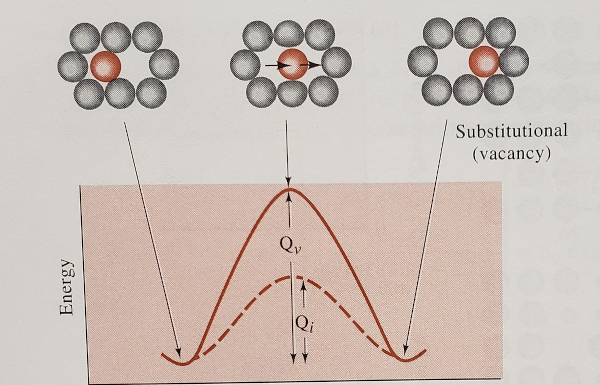
\includegraphics{figs/diffusion.png}
\caption{alt text}
\end{figure}

Consider how we might construct a simple model for tracer diffusion. As
an atom jumps from its site to an adjacent occupied site, it must
overcome a potential barrier, which depends on details of the local
crystallography and temperature. To calculate an absolute diffusion rate
requires then a determination of the activated jump process.

How can we model this? One could imagine using a method in which we
calculate all the forces between atoms and solve the equation of motion
of the atoms. This approach, called molecular dynamics, would give us
accurate diffusion constants, depending on the quality of the models used
to describe the interactions. We will cover the basics of molecular
dynamics in a later problem set. Another approach, called Kinetic Monte
Carlo, also incorporates details of interatomic interactions, but
requires a great deal of development before we can apply it.

Instead, we may turn to a simpler model to extract essential
characteristics of diffusion. The simplest of such models is a random
walk model, in which most of the details are ignored: there are no
interatomic interactions included in the model, the jump rates are
assumed to be the same for all possible jumps and the timescale is
measured relative to the jump rate, etc.

We start with a two-dimensional square lattice with one vacancy. One
could do a simulation in which we try to move all the atoms. Since only
those atoms next to a vacancy can move, it is equivalent to just move
the vacancy. We will do a random walk, by which we mean we shall let it
move around the system, where hops to any of the four nearest neighbors
is chosen by a random number. We will then measure the mean square
displacement $\langle r^2 \rangle$, which is related to the diffusion
constant.

$D = \frac{1}{6t}\langle r^2 \rangle$

Here we outline the basic approach for a random walk on a
two-dimensional square lattice. While we assume a square lattice, it is
important to note that in this approach, there is actually no lattice.
The symmetry is defined by the jumps. Thus, as we will find in following
exercises, extension to other crystal systems is straightforward.

In this class, we will use Python, an open-source object-oriented
programming language that is widely used in the materials science
community. Adaptation to other scientific programming languages such as
Fortran, C++, or MATLAB would be relatively straight forward.

    \hypertarget{random-walk-on-a-square-lattice}{%
\subsection{Random walk on a square
lattice}\label{random-walk-on-a-square-lattice}}

    \begin{tcolorbox}[breakable, size=fbox, boxrule=1pt, pad at break*=1mm,colback=cellbackground, colframe=cellborder]
\prompt{In}{incolor}{1}{\boxspacing}
\begin{Verbatim}[commandchars=\\\{\}]
\PY{c+c1}{\PYZsh{}\PYZsh{} Code for generating a single trajectory on square lattice}

\PY{c+c1}{\PYZsh{}\PYZsh{} a magic command that will transplant the *.py script directly as code}
\PY{c+c1}{\PYZsh{} \PYZpc{}load lattice\PYZus{}2D.py  }

\PY{c+c1}{\PYZsh{}\PYZsh{} a magic command that will show the contents of the *.py script}
\PY{c+c1}{\PYZsh{}\PYZsh{}   copy the code below into a file called lattice\PYZus{}2D.py in a folder called code\PYZus{}exercises}
\PY{c+c1}{\PYZsh{}\PYZsh{}   and reload this cell.}
\PY{o}{\PYZpc{}}\PY{k}{pycat} lattice\PYZus{}2D.py   
\end{Verbatim}
\end{tcolorbox}

    \begin{Shaded}
\begin{Highlighting}[]
\CommentTok{\# Random walk on a 2D lattice}

\ImportTok{import}\NormalTok{ numpy }\ImportTok{as}\NormalTok{ np}

\KeywordTok{def}\NormalTok{ random\_walk(nt,latt\_type):}
    \CommentTok{"""}
\CommentTok{    Random walk on a 2D lattice}
\CommentTok{    Inputs:}
\CommentTok{        nt [integer] = number of desired jumps (i.e., time steps)}
\CommentTok{        latt\_type [string] = lattice geometry, current options }
\CommentTok{                             are \textquotesingle{}square\textquotesingle{} and \textquotesingle{}triangle}
\CommentTok{    Outputs:}
\CommentTok{        rs2 [array] = square displacement at each time step}
\CommentTok{        x   [array] = x{-}coordinate at each time step}
\CommentTok{        y   [array] = y{-}coordinate at each time step}
\CommentTok{    """}
    \CommentTok{\# array for x{-} and y{-}coordinates along hopping path}
\NormalTok{    x }\OperatorTok{=}\NormalTok{ np.zeros(nt}\OperatorTok{+}\DecValTok{1}\NormalTok{)}
\NormalTok{    y }\OperatorTok{=}\NormalTok{ np.zeros(nt}\OperatorTok{+}\DecValTok{1}\NormalTok{)}
\NormalTok{    rs2 }\OperatorTok{=}\NormalTok{ np.zeros(nt}\OperatorTok{+}\DecValTok{1}\NormalTok{)}

    \CommentTok{\# particle starts at origin}
\NormalTok{    x[}\DecValTok{0}\NormalTok{] }\OperatorTok{=} \DecValTok{0} 
\NormalTok{    y[}\DecValTok{0}\NormalTok{] }\OperatorTok{=} \DecValTok{0}
\NormalTok{    rs2[}\DecValTok{0}\NormalTok{] }\OperatorTok{=} \DecValTok{0}

    \CommentTok{\#\# square lattice}
    \ControlFlowTok{if}\NormalTok{ latt\_type }\OperatorTok{==} \StringTok{\textquotesingle{}square\textquotesingle{}}\NormalTok{:}
        \CommentTok{\# create a list of random numbers from 1 to 4 with nt entries}
\NormalTok{        fd }\OperatorTok{=}\NormalTok{ np.floor(}\DecValTok{4} \OperatorTok{*}\NormalTok{ np.random.rand(nt))}
        \CommentTok{\# next two lines define the jumps on the square lattice:}
        \CommentTok{\#   right, up, left, down}
\NormalTok{        delx }\OperatorTok{=}\NormalTok{ np.array([}\DecValTok{1}\NormalTok{, }\OperatorTok{{-}}\DecValTok{1}\NormalTok{, }\DecValTok{0}\NormalTok{, }\DecValTok{0}\NormalTok{])}
\NormalTok{        dely }\OperatorTok{=}\NormalTok{ np.array([}\DecValTok{0}\NormalTok{, }\DecValTok{0}\NormalTok{, }\DecValTok{1}\NormalTok{, }\OperatorTok{{-}}\DecValTok{1}\NormalTok{])}
    \ControlFlowTok{else}\NormalTok{:}
        \ControlFlowTok{raise} \PreprocessorTok{ValueError}\NormalTok{(}\StringTok{"Lattice type not implemented! See random\_walk.py"}\NormalTok{)}
         
    \CommentTok{\# loop over nt jumps, add the jump vector as generated randomly in fd}
    \CommentTok{\#sum over nt jumps}
    \ControlFlowTok{for}\NormalTok{ j }\KeywordTok{in} \BuiltInTok{range}\NormalTok{(nt):}
\NormalTok{        x[j}\OperatorTok{+}\DecValTok{1}\NormalTok{] }\OperatorTok{=}\NormalTok{ x[j] }\OperatorTok{+}\NormalTok{ delx[}\BuiltInTok{int}\NormalTok{(fd[j])] }\CommentTok{\# x position at j+1 jump}
\NormalTok{        y[j}\OperatorTok{+}\DecValTok{1}\NormalTok{] }\OperatorTok{=}\NormalTok{ y[j] }\OperatorTok{+}\NormalTok{ dely[}\BuiltInTok{int}\NormalTok{(fd[j])] }\CommentTok{\# y position at j+1 jump}

        \CommentTok{\# square displacement position at j+1 jump in 2D}
\NormalTok{        rs2[j}\OperatorTok{+}\DecValTok{1}\NormalTok{] }\OperatorTok{=}\NormalTok{ x[j}\OperatorTok{+}\DecValTok{1}\NormalTok{]}\OperatorTok{**}\DecValTok{2} \OperatorTok{+}\NormalTok{ y[j}\OperatorTok{+}\DecValTok{1}\NormalTok{]}\OperatorTok{**}\DecValTok{2} 

    \ControlFlowTok{return}\NormalTok{ rs2, x, y}
\end{Highlighting}
\end{Shaded}

    The code is relatively straightforward. - We create a set of arrays that
will separately track the x- and y- coordinates - We initialize the
position of the random walker to be at the origin for the first step - A
list of $nt$ randomly-generated numbers between 1 and 4 is initialized
and will be used to choose the sequence of hops - We use the in-built
\texttt{numpy} function \texttt{random.rand} - \texttt{random.rand}
returns a list of random numbers between 0 and 1 (excluding 1) - Each
entry is multiplied by the number of nearest neighbors to return an
array of number between 0 and 4 (excluding 4) - In order to obtain of a
list of randomly-generated integers as indices for choosing each hop, we
use the \texttt{floor(x)} function, which rounds $x$ down to the
smaller integer.

For a square lattice, there are four possible jumps, given by four
vectors:

\begin{verbatim}
delx(0), dely(0) = (1,0) = right
delx(1), dely(1) = (-1,0) = left
delx(2), dely(2) = (0,1) = up
delx(3), dely(3) = (0,-1) = down
\end{verbatim}

In the \texttt{for} loop, we use the randomly-generated numbers in
\texttt{fd} to index \texttt{delx} and \texttt{dely} in order to choose
each subsequent hop, thus picking a random jump direction. The resulting
displacement described by \texttt{delx} and \texttt{dely} is added to
the current position. After each jump, the square displacement
\texttt{rs2} is computed. The user determines the total number of steps
taken in each trajectory by specifying \texttt{nt}. The function defined
for random walk on a square lattice returns the square of the
displacement \texttt{rs2} and the positions $(x,y)$ at each step.

The function \texttt{random\_walk\_square} computes one trajectory
(i.e., a sequence of jumps). In order to compute a mean square
displacement , we need to run many trajectories and average over them.

    \begin{tcolorbox}[breakable, size=fbox, boxrule=1pt, pad at break*=1mm,colback=cellbackground, colframe=cellborder]
\prompt{In}{incolor}{2}{\boxspacing}
\begin{Verbatim}[commandchars=\\\{\}]
\PY{c+c1}{\PYZsh{}\PYZsh{} Code for determining average mean square displacement over many trajectories }

\PY{c+c1}{\PYZsh{}\PYZsh{}   copy the code below into a file called avg\PYZus{}rand\PYZus{}walk2D.py in a folder called code\PYZus{}exercises}
\PY{c+c1}{\PYZsh{}\PYZsh{}   and reload this cell.}
\PY{o}{\PYZpc{}}\PY{k}{pycat} avg\PYZus{}rand\PYZus{}walk\PYZus{}2D.py
\end{Verbatim}
\end{tcolorbox}

    \begin{Shaded}
\begin{Highlighting}[]
\ImportTok{import}\NormalTok{ numpy }\ImportTok{as}\NormalTok{ np}
\ImportTok{from}\NormalTok{ lattice\_2D }\ImportTok{import}\NormalTok{ random\_walk}

\KeywordTok{def}\NormalTok{ avg\_rand\_walk(nt, nd, latt\_type):}
    \CommentTok{""" Average over many trajectories of random walkers}
\CommentTok{        Input:}
\CommentTok{            nt (integer) = number of jumps}
\CommentTok{            nd (integer) = number of trials }
\CommentTok{            latt\_type (string) = type of lattice,}
\CommentTok{                                 "square" or "triangular" implemented}
\CommentTok{        Output:}
\CommentTok{            rwa (list; float) = mean square displacement of each trajectory}
\CommentTok{            ree (list; float) = end{-}to{-}end distance for each trial}
\CommentTok{            sig (list; float) = relative standard deviation of \textless{}r\^{}2\textgreater{}}
\CommentTok{                                of each trajectory}
\CommentTok{    """}

    \CommentTok{\# Initialize the variables for calculating \textless{}R\^{}2\textgreater{} and \textless{}R\^{}4\textgreater{}}
\NormalTok{    rwa }\OperatorTok{=}\NormalTok{ np.zeros(nt}\OperatorTok{+}\DecValTok{1}\NormalTok{)}
\NormalTok{    ree }\OperatorTok{=}\NormalTok{ np.zeros(nd)}
\NormalTok{    sig }\OperatorTok{=}\NormalTok{ np.zeros(nt}\OperatorTok{+}\DecValTok{1}\NormalTok{)}

    \CommentTok{\# Loop over trials}
    \ControlFlowTok{for}\NormalTok{ j }\KeywordTok{in} \BuiltInTok{range}\NormalTok{(nd):}
        \CommentTok{\# Call random walker code from above to generate a trajectory}
\NormalTok{        g, x, y }\OperatorTok{=}\NormalTok{ random\_walk(nt,latt\_type)}

        \CommentTok{\# Calculate end{-}to{-}end distance, 2D}
        \CommentTok{\# index last element}
\NormalTok{        ree[j] }\OperatorTok{=}\NormalTok{ np.sqrt(x[}\OperatorTok{{-}}\DecValTok{1}\NormalTok{]}\OperatorTok{**}\DecValTok{2} \OperatorTok{+}\NormalTok{ y[}\OperatorTok{{-}}\DecValTok{1}\NormalTok{]}\OperatorTok{**}\DecValTok{2}\NormalTok{ )}

        \CommentTok{\# Increment R\^{}2 and R\^{}4 at each time step (jump)}
        \ControlFlowTok{for}\NormalTok{ k }\KeywordTok{in} \BuiltInTok{range}\NormalTok{(nt}\OperatorTok{+}\DecValTok{1}\NormalTok{):}
\NormalTok{            rwa[k] }\OperatorTok{+=}\NormalTok{ g[k]}
\NormalTok{            sig[k] }\OperatorTok{+=}\NormalTok{ g[k] }\OperatorTok{**} \DecValTok{2}

    \CommentTok{\# Find averages by dividing by the number of trials}
    \CommentTok{\# Note: rwa[0] is 0 by definition, will throw a NaN warning }
    \ControlFlowTok{for}\NormalTok{ k }\KeywordTok{in} \BuiltInTok{range}\NormalTok{(nt}\OperatorTok{+}\DecValTok{1}\NormalTok{):}
\NormalTok{        rwa[k] }\OperatorTok{/=}\NormalTok{ nd}
\NormalTok{        sig[k] }\OperatorTok{=}\NormalTok{ (sig[k] }\OperatorTok{/} \BuiltInTok{float}\NormalTok{(nd) }\OperatorTok{{-}}\NormalTok{ rwa[k] }\OperatorTok{**} \DecValTok{2}\NormalTok{) }\OperatorTok{/}\NormalTok{ rwa[k] }\OperatorTok{**} \DecValTok{2}

    \ControlFlowTok{return}\NormalTok{ rwa, ree, sig}
\end{Highlighting}
\end{Shaded}

    \hypertarget{exercises}{%
\subsection{============= Exercises ==============}\label{exercises}}

    \hypertarget{random-walk-on-different-types-of-lattices}{%
\subsubsection{Random walk on different types of
lattices}\label{random-walk-on-different-types-of-lattices}}

In these exercises, there is no prescription on how to organize your
code, but it is highly recommended that you think about how to organize
your code and anticipate modifications of new additions to the code.

\begin{enumerate}
\def\labelenumi{\arabic{enumi}.}
\tightlist
\item
  Consider a random walk on a 2D square lattice:\\

  \begin{enumerate}
  \def\labelenumii{\alph{enumii}.}
  \tightlist
  \item
    Use the code provided or write a new one and run it.\\
  \item
    Plot at least two trajectories and compare.\\
  \item
    Calculate the mean square displacement. Examine the behavior of the
    mean square displacement for a single run and for many runs.\\
  \item
    How many runs are needed to obtain a straight line for the mean
    square displacement?
  \end{enumerate}
\end{enumerate}

    \begin{enumerate}
\def\labelenumi{\arabic{enumi}.}
\setcounter{enumi}{1}
\tightlist
\item
  Modify the code such that diffusion occurs on a 2D triangular lattice.
  Repeat the questions in 1. How do the results compare?
\end{enumerate}

    \begin{enumerate}
\def\labelenumi{\arabic{enumi}.}
\setcounter{enumi}{2}
\tightlist
\item
  Modify the code such that diffusion occurs on a 3D simple cubic
  lattice. Repeat the questions in 1. How do the results compare?
\end{enumerate}

    \begin{enumerate}
\def\labelenumi{\arabic{enumi}.}
\setcounter{enumi}{3}
\tightlist
\item
  Modify the code such that diffusion occurs on a 3D face-centered cubic
  lattice. Repeat the questions in 1. How do the results compare?
\end{enumerate}

    \hypertarget{statistics-of-the-random-walk-model}{%
\subsubsection{Statistics of the random-walk
model}\label{statistics-of-the-random-walk-model}}

Consider 1D diffusion along the $x$-axis starting at $x = 0$ in step
sizes of $a$. There is an equal probability the particle will hop to
the left or right. After $n$ jumps, we will record a final position
$x_n$. Suppose we generate many such trajectories and average over
them to find the probability of the particle at $x_n$ along the 1D
lattice. The probability of finding the particle at $x_n$ would have
the functional form of a Gaussian distribution.

$I(x_n) = \Big(\frac{3}{2\pi n a^2}\Big)^{1/2} \exp\Big(-\frac{3x_n^2}{2n a^2}\Big)$

In three-dimensions, the corresponding probability distribution of the
position is given by

$\mathcal{P}(\textbf{R}_n) = I(x_n)I(y_n)I(z_n)$

where $\textbf{R}_n = (x_n, y_n, z_n)$ and $I(y_n)$ and $I(z_n)$
have expressions similar to $I(x_n)$.

A more useful quantitify would be the probability distribution of the
end-to-end distance $R_n = |\textbf{R}_n|$, i.e., a measure of how far
the atom particle has diffused in $n$ steps. To find
$\mathcal{P}(R_n)$, the angular information contained in the
distribution of $\textbf{R}_n$ vectors must be averaged out, which can
be accomplished by tranforming to spherical polar coordinates and
integrating out the angles. Once that is done, we find the probability
distribution of the end-to-end distance in 3D is

\begin{equation}
\mathcal{P}(R_n) = \Big(\frac{3}{2\pi n a^2}\Big)^{3/2} 4\pi R_n^2 \exp\Big(-\frac{3R_n^2}{2n a^2}\Big)    
\end{equation}


\begin{enumerate}
\def\labelenumi{\arabic{enumi}.}
\setcounter{enumi}{4}
\tightlist
\item
  Make separate plots showing $I(x_n)$ and $\mathcal{P}(R_n)$.
  Provide a physical interpretation of the plot of $I(x_n)$ at large
  negative $-x_n$ values. How does the most probable point for
  $I(x_n)$ compare with that of $\mathcal{P}(R_n)$?
\end{enumerate}

Supposed we have $m$ random-walk simulations giving us $m$ values
for $R_n$ after $n$ jump sequences. Create a discrete representation
of $\mathcal{P}(R_n)$ for a specific set of values of $R_n$ by
dividing the $m$ values into user-defined bins that represent a
finite-range of $R_n$. In other words, create histogram by breaking up
the data into $n_{bin}$ equally-spaced bins with bin width

\begin{equation}
\Delta = \frac{R_n^{max} - R_n^{min}}{n_{bin}}    
\end{equation}


Then determine $m_i$, number of $R_n$ that lies within each $i$th
bin. The probability of a value $R_n$ is thus

\begin{equation}
\mathcal{P}_i = m_i/m
\end{equation}

\begin{enumerate}
\def\labelenumi{\arabic{enumi}.}
\setcounter{enumi}{5}
\tightlist
\item
  Run a series of trajectories and implement a binning procedure to
  calculate the probability distribution of the end-to-end distance
  across a series of trajectories. Compare your histogram of $R_n$
  from your computed trajectories with the predicted form of
  $\mathcal{P}(R_n)$.

  \begin{enumerate}
  \def\labelenumii{\alph{enumii}.}
  \tightlist
  \item
    how many runs are needed to obtain well-converged results?
  \item
    how many bins are needed to obtain fine enough resolution?
  \end{enumerate}
\end{enumerate}


    % Add a bibliography block to the postdoc
    
    
    
\end{document}
